\documentclass[10pt, twocolumn]{IEEEtran}
% Leaving this next line in to periodically check how many Normal People Pages were written
%\documentclass[12pt, letterpaper]{article}
\usepackage[utf8]{inputenc}

\usepackage{listings}
\usepackage{xcolor}

\definecolor{codegreen}{rgb}{0,0.6,0}
\definecolor{codegray}{rgb}{0.5,0.5,0.5}
\definecolor{codepurple}{rgb}{0.58,0,0.82}
\definecolor{backcolour}{rgb}{0.95,0.95,0.92}

\lstset{
	language=c++,
	backgroundcolor=\color{backcolour},   
	commentstyle=\color{codegreen},
	keywordstyle=\color{magenta},
	numberstyle=\tiny\color{codegray},
	stringstyle=\color{codepurple},
	basicstyle=\ttfamily\footnotesize,
	breakatwhitespace=false,         
	breaklines=true,                 
	captionpos=b,                    
	keepspaces=true,                 
	numbers=left,                    
	numbersep=5pt,                  
	showspaces=false,                
	showstringspaces=false,
	showtabs=false,                  
	tabsize=2
}

\usepackage{graphicx}
\usepackage{mathtools}

\usepackage[style=apa, backend=biber]{biblatex}
\addbibresource{paper.bib}

\title{Granular Synthesis for Instrument Makers}
\author{	
	\IEEEauthorblockN{Daniël Kamp\\}
    \IEEEauthorblockA{HKU University of the Arts Utrecht
    \\daniel.kamp@student.hku.nl}
    }
\date{April 2022}

\begin{document}

\maketitle

\begin{abstract}
This writing sheds light onto various forms of granular synthesis. It analyses some existing implementations, explains the inner workings of such a system, and provides insight into human interfaces to use this method of sound generation.
\end{abstract}

\section*{Introduction}
Granular synthesis is a versatile form of sample-based (digital) sound synthesis. It uses short slices of recorded audio to create new, rich sounds. These slices can be layered, stretched, spread, and in other ways processed to create vast soundscapes with relative ease. \\
This writing aims to demystify the technical aspects of granular synthesis, and provide a comprehensive insight for instrument makers who want to make use of the technique.

\section{What is granular synthesis?}
This first part tells a brief history of granular synthesis, explains the components of a system implementing this technique, and lists some reference instruments.

\subsection{A brief history}
Granular synthesis as it's known today is a form of digital sound synthesis, which is based on the processing of small slices of sampled audio known as "grains". The underlying view on sound perception was first proposed by Hungarian-British physicist Dennis Gabor in an article titled \textit{Acoustical Quanta and the Theory of Hearing} (\cite{gabor47}). In this writing, Gabor theorized an approach to sound similar to concepts found in quantum mechanics.\\ Building on this theory, in the late 1950s, Greek composer Iannis Xenakis started experimenting with the technique, stitching together many tiny slices of tape to create new sounds (\cite{robindore96}). Inspired by Xenakis during a 1972 workshop taught by the former, composer Curtis Roads eventually created the first computer software implementing this synthesis paradigm in 1974 (\cite{opie03}). His code produced a 30-second long piece titled Klang-1, using three parameters: envelope, duration, and density. This software, however, did not operate in real-time, and producing this piece of music took multiple days. The first real-time implementation of the principle came from Canadian composer Barry Truax, who developed GSX (1986) and GSAMX (1987) (\cite{truax88}). \\
Since then, granular synthesis has established itself as a pillar of modern digital sound generation. More approachable implementations of the technique, like Robert Henke's Granulator (2011), made it possible for anyone with a computer to explore its vast new possibilities in sound. Today, dozens of granular synthesizers are available, each offering a different approach to a 75-year-old concept.

\subsection{General system overview}
This section describes the general anatomy of a granular synthesizer, and gives a broad overview of the building blocks that make up such a system. 

\begin{figure}[ht!]
	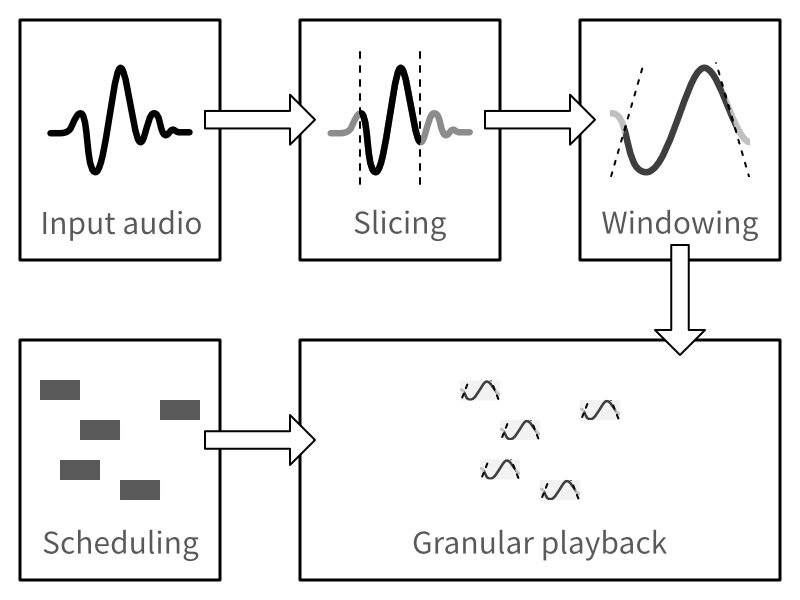
\includegraphics[width=\linewidth]{GranularDiagram.png}
	\caption{A simplified overview of a granular synthesis system.}
	\label{fig:block_diagram}
\end{figure}

\subsubsection{Sound source}
As its input, a granular system takes a sound stream. This stream can consist of sampled audio, live microphone input, or generated audio (such as sine waves). The content of this source material has an effect on the sounds one can generate: [insert comparison: transient-rich vs low-activity].

\subsubsection{Models}
There are four distinguishable models of granular synthesis: screen, cloud, stream, and spray (\cite{roads12}). The first of these, screen, was described by Xenakis and would run a series of time-frequency plots at a fixed time rate (\cite{xenakis63}). In layman's terms, this would be comparable to a flip book animation, used for sound instead. \\
The second model, clouds, generates a cloud of sound in which the individual grains are not bound to predefined parameters, but instead spread across specified ranges in a stochastic manner. This creates rich, unpredictable textures that are often used on a macro level within compositions. \\
The more regular counterpart of clouds is streams, in which grains are distributed in a deterministic process. In this model, the density (number of grains per second) determines a regular interval at which grains are played, creating a sort of rhythmic texture. This rhythm can be tweaked by modifying the grain density, through which one can create tone-like sounds. \\
A model that is used in modern digital granular synthesis is spray. This implementation makes it possible for users to draw the grains on a plot of frequency over time, which makes for an intuitive interaction model.

\subsubsection{Windowing and envelope}
Since the start position of grains is rather arbitrary, there is no telling what the amplitude of the first sample in the selection will be. Therefore, it's good practice, as it is in any digital audio application, to apply an envelope that trims off any rough edges that may exist in the source material. This envelope can be modified to a user's own insight through the parameters \textit{shape} and \textit{length}. \\
The shape of an envelope refers to its mathematical function. In this regard, there are four commonly used shapes: linear, square root, exponential, and Gaussian. The latter was proposed by Dennis Gabor in his original theory on granular sound, and is still commonly used. More recently, due to developments in the field of processing power in computers over the past fifty-or-so years, it has become possible and commonplace to use other envelope shapes as well. Figure \ref{fig:env_shapes} shows the four functions as a plot of amplitude over time.

\begin{figure}[ht!]
	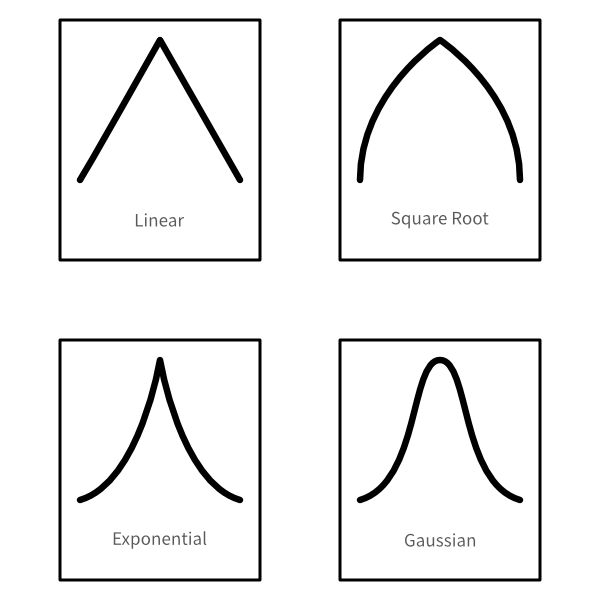
\includegraphics[width=\linewidth]{env_shapes.png}
	\caption{Four envelope shapes.}
	\label{fig:env_shapes}
\end{figure}

The length of an envelope simply describes the time it takes for the signal to reach its full amplitude. By varying this number, one can change the character of the resulting sound. If a long \textit{attack} (rising edge of the envelope) is used, the resulting audio will sound more mellow compared to when a short attack time is applied.

\subsubsection{Duration and density}
Density, as mentioned previously, describes the number of grains played in one (1) second. Variations in this domain can roughly be split into two categories: \textit{deterministic} and \textit{stochastic}.\\
In a deterministic distribution, grains are played back with even spacing between them. This means that the resulting sound is of a regular nature. For example, this method would produce audio in which a grain is played every 100 ms. \\
Stochastic distribution, on the other hand, adds a realm of uncertainty to the sound. When this distribution is applied, the beginning and length of each grain are randomized. This means that the resulting sound is no longer predictable and/or regular in nature. Using this method, one can create vast clouds of sound that contain no structure or repetition.

\subsection{Existing instruments}
This section lists a few instruments and effects that use granular synthesis. \\
\textit{Author's note:} I selected open-source instruments of which the source code is freely available to the public. This way, I can give an in-depth comparison of the inner workings of these instruments. I'll use these and their concrete implementations as references throughout the rest of my research described in this writing.

\subsubsection{Mutable Instruments' Clouds}
Clouds is a Eurorack module developed and produced by Émilie Gillet (Mutable Instruments). Both the hardware files (schematics, CAD-files) and firmware source code are open-source and publicly available (\cite{clouds}).\\
As its source sound, Clouds uses incoming stereo audio compliant with the Eurorack standard.\\
Looking at the source files of Clouds, one can dissect the process used to "seed" grains. First, a maximum number of grains is "hard-coded" into the software. The program will create new ones until this limit is reached. Clouds offers both deterministic and stochastic seeding modes, which can be selected by the user. In deterministic mode, one controls the time between seeds in a regular manner. In stochastic mode, the user input controls the likelihood with which grains will be created.\\
This implementation uses so-called Look Up Tables (LUTs) to store data for its envelopes and other resource-intensive processes. These tables contain pre-calculated numbers, so that the program doesn't need to calculate these in real-time. This makes it suitable for low-power devices (in case of Clouds, this is an STM32 micro-controller). The next chapter contains examples of, and a comparison between this implementation and one that does calculate its data in real-time.

\subsubsection{Argotlunar}
Argotlunar is a real-time granular VST and AudioUnit plugin created by Michael Ourednik. The source code of this software is open-source and available via GitHub (\cite{argotlunar}).


\section{How does granular synthesis work?}
This part dives deeper into the inner workings of a granular system. Starting with a brief explanation of core audiological concepts that define how we experience sound on a short time scale, it then proceeds to explain concrete implementations of a granular synthesizer in C++. These examples are then compared through statistics about their performance, so a recommendation can be made based on system efficiency.

\subsection{Audiological concepts}
Here I SHORTLY describe the audiological concepts that make this system possible. AKA: why do we perceive lots of small ticks as a coherent sound, and IMPORTANT: what criteria does our system need to fit in order to be deemed a successful granular synthesizer. This makes our hypothesis concrete and closed off.

\subsection{Implementations}
In this section, implementations and methods are proposed for specific parts of the system. The next section will take execution metrics from these example implementations, and validate them by the requirements defined previously.

\subsubsection{Sound sourcing and selection}
This part lists different methods of sound sourcing and sample selection:
- Microphone or audio input
- Sample-based granular synthesis\\
For sample selection:
- Randomized selection
- Transient selection
\subsubsection{Trigger algorithms}
This section gives three examples of grain trigger algorithms, using two different approaches. These algorithms determine when grains are played, and thus heavily influence the character of the resulting sound.\\

\textbf{Deterministic approach}\\
For a deterministic method, a user directly or indirectly controls the sound's \textit{density}, using parameters like \textit{grain length} and \textit{grain interval}. Playing back grains with a regular interval creates a predictable and periodic output sound, which can even be used in a melodic way. The following code example implements a deterministic approach for a single stream of grains.
\begin{lstlisting}[caption={A deterministic method of grain "seeding"}]
	// User parameter input
	float density = 0.5;
	int grain_length = 100;
	
	// Calculate the interval with which grains are triggered
	int interval = (float) grain_length / 0.5;
	
	// Iterate and trigger grains
	for(int i = 0; i < block_size; i++) {
		if(!(i % interval)) {
			grains.push_back(new Grain {start: i});
		}
	}
\end{lstlisting}

\textbf{Stochastic implementation 1: using \lstinline|std::rand()|}\\
To add variation to a sound, one might want to depart from a periodic triggering algorithm like the one described above. The cloud model, as mentioned in section 1.B, exchanges the regular interval for random chance. \\
To give a user more control, a program implementing this method might provide an offset control that limits the rate at which new grains are created. \\


\textbf{Stochastic implementation 2: using \lstinline|<random>|}\\
For basic randomness, using \lstinline|std::rand()| will usually suffice. However, for more control over the stochastic process, one may choose to use a more sophisticated algorithm. The C++ Standard Library includes some alternative implementations that may be used in this scenario.\\

\textbf{Stochastic implementation 3: using a Look-Up Table}\\
On low-power devices, one might consider populating a table with noise beforehand, and embedding it into the program.\\ 

\subsubsection{Windowing algorithms and approaches}
This section compares three approaches for implementing an envelope generator. For simplicity, each method renders a quadratic parabola envelope shape with a duration of 4096 samples.  \\

\textbf{First implementation: Pre-rendering}\\
This method calculates a new lookup table when any values (such as envelope or grain length) are changed. This way, the program can simply look up and apply the right value during the rendering process, without needing additional calculations.
\begin{lstlisting}[caption={Envelope application using a pre-rendering algorithm}]
	#define ENV_ROUNDS 4096
		
	float envelope[ENV_ROUNDS];
	float intermediate_;
		
	// Initialization, runs once
	for(int i = 0; i < ENV_ROUNDS; i++) {
		intermediate_ = ENV_SHAPE * (float)(-1.0 * i * i + ENV_ROUNDS * i);
		envelope[i] = (intermediate_ >= 1.0) * 1.0 + (intermediate_ < 1.0) * intermediate_;
	}
		
	// Rendering loop, runs while active
	for(int i = 0; i < ENV_ROUNDS; i++) {
		test1[i] = sample[i] * envelope[i];
	}
\end{lstlisting}

\textbf{Second implementation: Look-Up Table}\\
In this next example, the program first scales its position in relation to the generated look-up table. Using this scaled position, it looks up the nearest corresponding value. It then uses a low pass filter to interpolate between the current and previous value.\\
The following formula was used to generate the data for the look-up table:
\[
y_n(x_n) = \frac{0.001*((-x_n^2)+\textit{grain size}*x_n)}{\textit{grain size}}
\]
\[	
f_n(y_n) = \frac{3}{2} * \begin{cases}
	\frac{y_n^3}{3}  	& y_n < 1.0 \\
	\frac{2}{3} 	& y_n \geq 1.0
\end{cases}
\]
\begin{lstlisting}[caption={Envelope application using a look-up table}]
	// Initialization, runs once
	float ENVELOPE_LUT[6000] = {0, 0.00149975, 0.002998996, 0.004497737, ...};
	
	auto scale_factor = (sizeof(ENVELOPE_LUT) / sizeof(ENVELOPE_LUT[0])) / ENV_ROUNDS;
	float previous = ENVELOPE_LUT[0];
	int ptr = 0;
	float tmp = 0.0;
	
	// Rendering loop, runs while active
	for(int i = 0; i < ENV_ROUNDS; i++) {
		ptr = floor(scale_factor * i);
		
		tmp = 0.5 * (envelope[ptr] + previous);
		test2[i] = tmp * sample[i];
		
		previous = envelope[ptr];
	}
\end{lstlisting}

\textbf{Third implementation: Real-Time Rendering}\\
This last example is taken directly from the Argotlunar source code. It calculates a step and slope value, and uses these to increment the envelope's multiplication variable.

\begin{lstlisting}[caption={Envelope application using real-time rendering}]
	// Code by M. Ourednik
	// Initialization, runs once
	float env_amp = 0.0f;
	float d = 1.0f / ENV_ROUNDS;
	float d2 = d * d;
	float slope = 4.0f * 0.8 * (d - d2);
	float curve = -8.0f * 0.8 * d2;
	
	// Rendering loop, runs while active
	for (int i = 0; i < ENV_ROUNDS; i++) {
		env_amp += slope;
		slope += curve;
		test3[i] = sample[i] * env_amp;
	}
\end{lstlisting}


\subsection{Efficiency}
For this section, the implementations from above were ran multiple times, to gain an accurate result. The execution time of each loop iteration has been recorded, along with the initialization time. Note that these benchmarks were ran on a 2019 MacBook Pro (Intel Core i7 6-core processor, 16GB RAM).

\subsubsection{Trigger algorithms}
The first results describe the performance of the trigger algorithms proposed earlier. These implementations are compared not by execution time necessarily, but more so by adherence to a user's intention. For example, if a user turns the density knob, the resulting sound should reflect the desired changes.

\subsubsection{Envelopes}
Next, the benchmark results of the envelope implementations show some interesting details. Before looking at the runtime statistics, let's analyze the initialization times of each algorithm. Figure \ref{fig:env_init_time} shows this data, measured in nanoseconds.

\begin{figure}[ht!]
	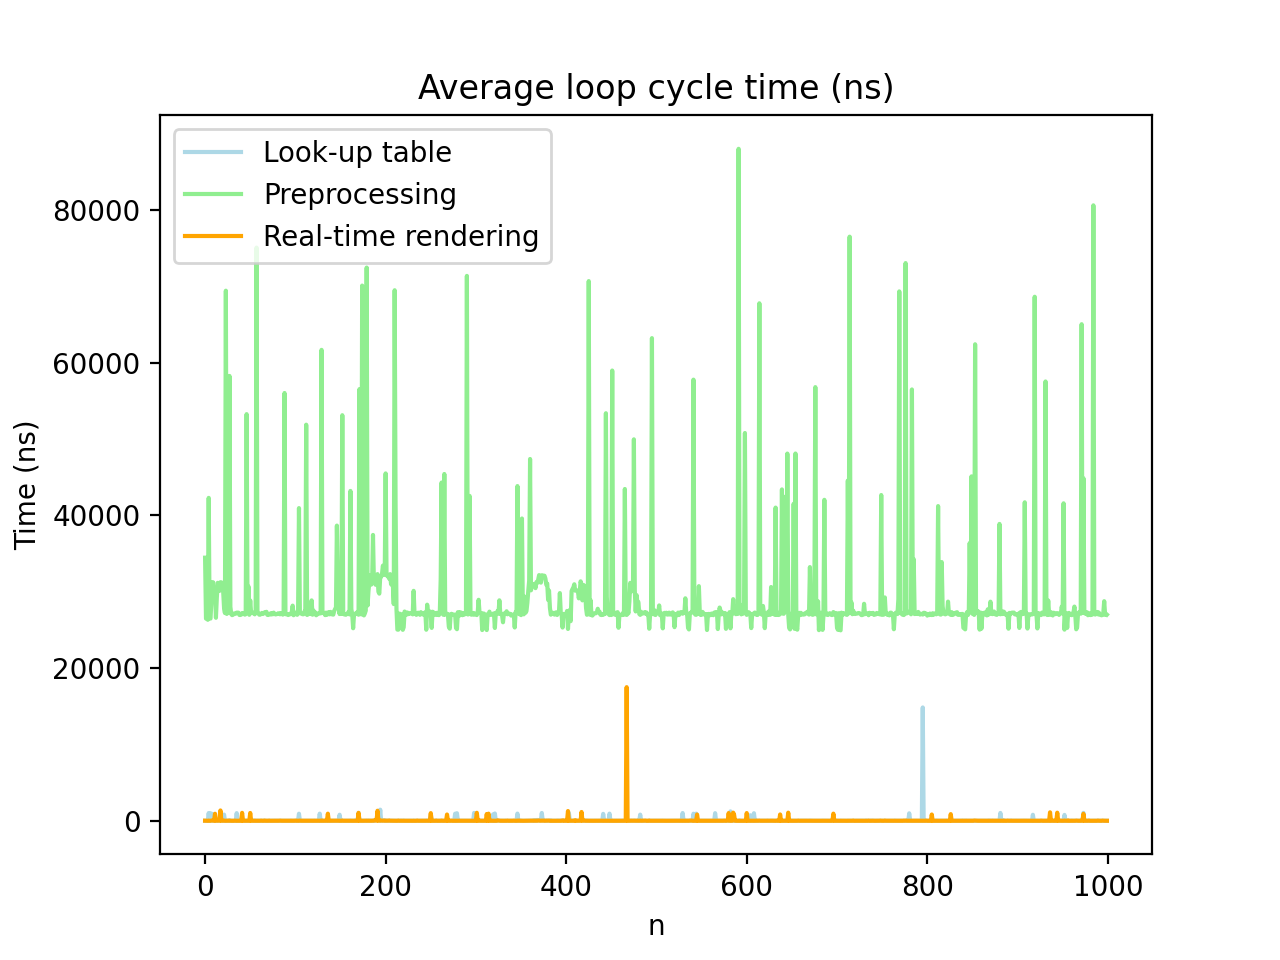
\includegraphics[width=\linewidth]{env_init_time.png}
	\caption{Initialization time, measured 100 times.}
	\label{fig:env_init_time}
\end{figure}

Looking at this graph, one will notice that the pre-processing implementation takes significantly longer to initialize than its counterparts. This can be attributed to the way this method renders its data all at once during this initialization phase.\\
The second graph, however, paints a different picture. Comparing the results in Figure \ref{fig:env_average_cycle_time}, both the pre-processing and real-time algorithm have an average render cycle time of around 42ns, while the look-up table method takes over 10ns longer.

\begin{figure}[ht!]
	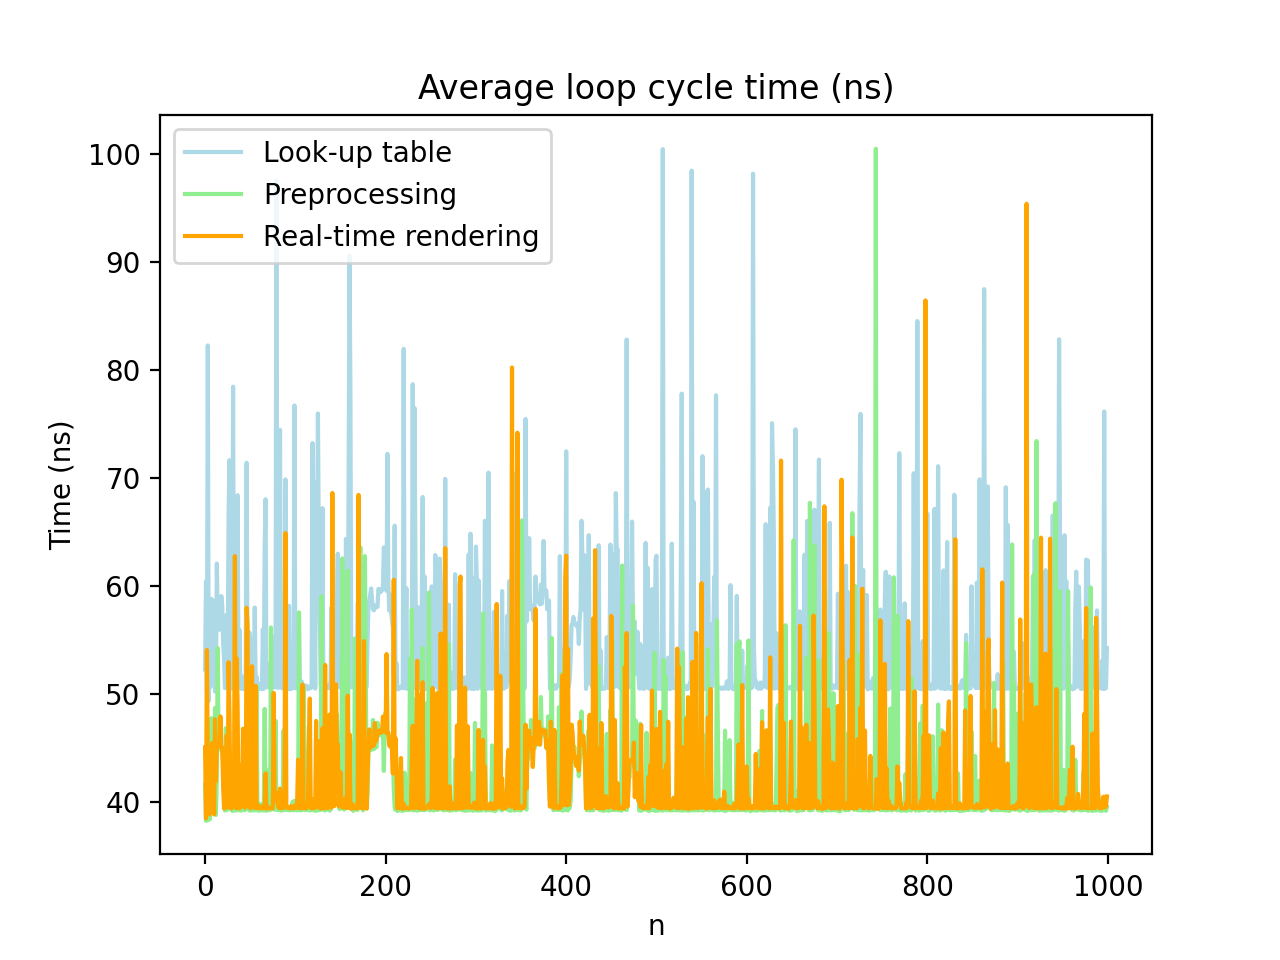
\includegraphics[width=\linewidth]{env_average_cycle_time.png}
	\caption{Average time per rendering cycle, measured 1000 times.}
	\label{fig:env_average_cycle_time}
\end{figure}

\section{How is granular synthesis used?}
This section looks at the human aspect of granular synthesis: what sounds does it produce, how is it controlled, and how can one play an instrument that uses this technique. KEEP THIS PART SHORT

\subsection{Human control}
This subsection looks at ways a human being can control a granular instrument. Common input methods like touch interfaces, sliders, knobs, and digital UIs are described and compared.

\subsection{Playability}
This subsection looks at how such instruments can be controlled in an artistic manner. It provides an insight into live performance methods and some useful macros (maybe).

\section*{Conclusions}
This section summarizes my findings from the research, and gives a careful recommendation on implementing such system based on these results.

\printbibliography
\textit{All graphics in this writing were created by the author, unless otherwise noted.}

\end{document}